\documentclass{article}

\usepackage[a4paper, bottom=0.5in, top=0.5in, left=0.5in, right=0.5in]{geometry}
\usepackage{wrapfig}
\usepackage{natbib}
\usepackage{url}
\usepackage{xcolor}
\usepackage{caption}
\usepackage{hyperref}
\hypersetup{
    colorlinks=true,    
    urlcolor=cyan,
}
\usepackage{bytefield}

\usepackage{amsfonts}
\usepackage{float}
\usepackage{enumitem}



\newcommand{\bitFormat}[1]{\emph{\textbf{\textcolor{cyan}{#1}}}}

\newcommand{\regFormat}[1]{\textbf{\textcolor{magenta}{#1}}}

\newcommand{\pinFormat}[1]{\emph{\textcolor{red}{#1}}}


\usepackage{graphicx}
\graphicspath{ {./Resources/pics/} }



\title{ATmega328P Basics}
\author{Narendiran S}
\date{\today}

\begin{document}
\maketitle

\section{Features}
\begin{itemize}
    \item 8 bit CMOS $\mu$C with RISC Architecture
    \item 32 x 8-bit General purpose registers
    \item 32 KByte of flash program memory
    \item 1 KByte EEPROM
    \item 2 KByte of internal SRAM
    \item On-chip 2-cycle multiplier
    \item Optional boot code section with independent lock bits
    \begin{itemize}
        \item In-system programming by on-chip boot program
        \item True read-while-write operation
    \end{itemize}
    \item Two 8-bit Timer/Counter with  separate prescaler and compare mode
    \item One 16-bit Timer/Counter with  separate prescaler, compare mode and capture mode
    \item Real time counter with separate oscillator
    \item Six PWM channels
    \item 6/8(DEPENDING ON PACKAGE) chaneel 10 bit ADC 
        ◦ Also with Temperature measurement
    \item Programmable serial USART
    \item 2-wire serial interface (Phillips I2C compatible)
    \item Programmable watchdog timer with separate on-chip oscillator
    \item On-chip analog comparator
    \item Interrupt and wake-up on pin change
    \item Power-on reset and programmable brown-out detection
    \item External and internal interrupt sources
    \item Six sleep modes: Idle, ADC noise reduction, power-save, power-down, standby  and external standby
    \item 2.7V to 5.5V for ATmega328P
\end{itemize}

\newpage
\section{Block Diagram}
\begin{figure}[H]
    \centering
    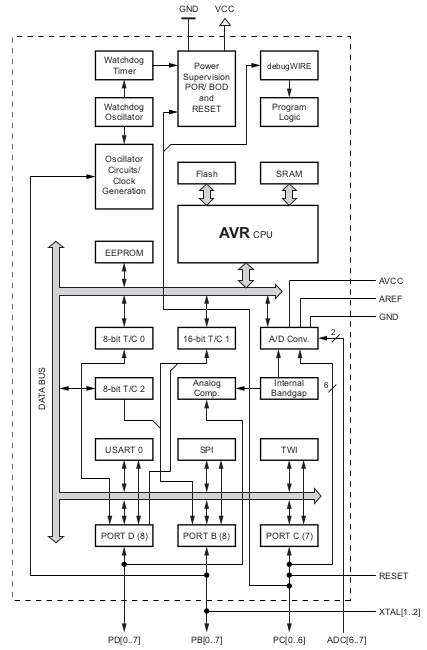
\includegraphics{blockDiagram.png}
\end{figure}

\newpage
\section{Pins}
\subsection{Power Pins}
\quad VCC, Gnd - 2.7V to 5.5V

\subsection{PORTB - PB7:PB0}
\begin{itemize}
    \item Bidirection I/O with internal pull-up resistor(selectable for each bit)
    \item Tristate when reset
    \item Depending on the clock selection fuse settings,
    \begin{itemize}
        \item \pinFormat{PB6} – input of inverting oscillator amplifier and input to internal clock operating circuit
        \item \pinFormat{PB7} – output of inverting oscillator amplifier
    \end{itemize}
    \item If internal calibrated RC oscillator is used as clock source, \pinFormat{PB7} and \pinFormat{PB6} is used as \pinFormat{TOSC2} and \pinFormat{TOSC1} input for Timer/Counter2
\end{itemize}

\subsection{PORTC - PC5:PB0}
\begin{itemize}
    \item Bidirection I/O with internal pull-up resistor(selectable for each bit)
    \item Tristate when reset
\end{itemize}

\subsection{PC6/\texorpdfstring{$\overline{RESET}$}{}}
\begin{itemize}
    \item Low level on this pin will gnerate reset, even if no clock running.
    \item \bitFormat{RSTDIBL} fuse == programmed(0) -- \pinFormat{PC6} is input pin.
    \item \bitFormat{RSTDIBL} fuse == unprogrammed(1) -- \pinFormat{PC6} is reset pin.
\end{itemize}

\subsection{PORTD - PD7:PD0}
\begin{itemize}
    \item Bidirection I/O with internal pull-up resistor(selectable for each bit)
    \item Tristate when reset
\end{itemize}

\subsection{\texorpdfstring{$AV_{CC}$}{}}
\begin{itemize}
    \item Supply voltage pin for A/D converter
    \item Connected to External Vcc when not used
    \item Connected to Vcc through LPF when used
\end{itemize}

\subsection{AREF}
\quad Analog reference pin of A/D Converter

\subsection{ADC7:ADC6}
\quad Analog input to ADC(10bit ADC)


\section{Modes}
\subsection{Idle Mode}
\quad Stops the CPU while allowing SRAM, TImer/Counters, USART, 2-wire serial interface, SPI port and interrupt system to continue functioning.

\subsection{Power-Down Mode}
\quad Saves the register contents but freezes the oscillator, disabling all other chip functions untill next interrupt or hardware reset.

\subsection{Power-Save Mode}
\quad The asynchonous timer continues to run, allowing user to maintain timer base while reset of devices is sleeping.

\subsection{ADC Noise reduction mode}
\quad Stops CPU and all I/O modules except asynchonous timer and ADC to minimize switching noise during ADC conversions.

\subsection{Standby Mode}
\quad The crystall/oscillator is running while reset of devices is sleeping. Allows very fast start-up combined with low power consumption.


\section{AVR CPU Core}
\quad The main function of CPU core is access memory, perform caluclations, control peripherals and handle interrupts.

\begin{figure}[H]
    \centering
    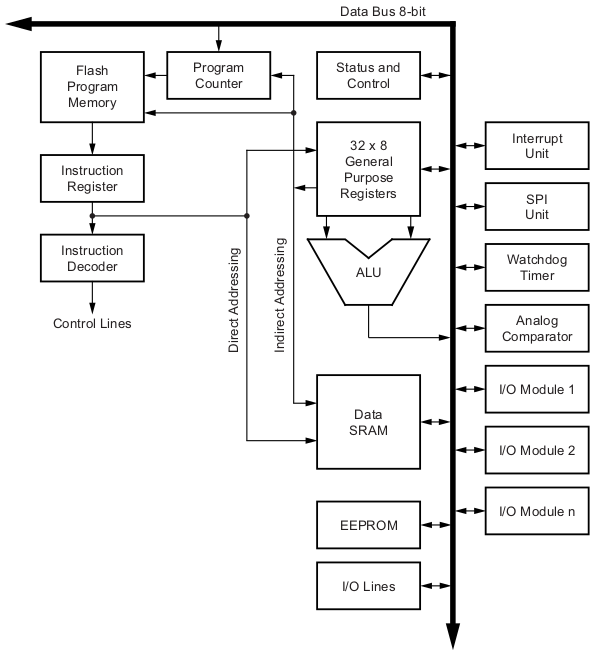
\includegraphics[height=0.7\textheight]{avrCoreBlockDiagram.png}
\end{figure}

\begin{itemize}
    \item For performance and parallelism, the AVR uses Harvard Architecture - with seperate memories and buses for program and data.
    \item Instructions in Program memory are exectued with a single level pipelining.
    \item The program memory is  \textbf{In-system Reprogrammable Flash memory}.
    \item The register file consist of 32 x 8-bit General Purpose Registers with a single clock cycle assess time.
    \item One ALU operation uses two operatands from register file and store back the result to register file in one clock cycle.
    \item Six 32-bit register combine to form the X-, Y- and Z- registers which help in 16-bit indirect address register pointer for data space.
    \item One of these pointers acts as address pointer for look-up tables in Flash Program Memory.
    \item Program memory adress cotains 16-bit or 32-bit Instructions.
    \item Program Flash memory space is divided into two sections - each section have dedicated lock bits for read/write protection.
    \begin{itemize}
        \item Boot Program section
        \item Application Program section
    \end{itemize}
    \item I/O memory space contains 64 addresses for CPU peripheral functions as control register, SPI and Other I/O functionscan be accessed directly or through register file from 0x20 - 0x5F.
    \item Has extended I/O space from 0x60 - 0xFF in SRAM.
\end{itemize}

\subsection{Reset and Interrupt vectors}
\begin{itemize}
    \item Interrupts and reset vectors have seperate program vecotr in program memory space.
    \item Interrupts maye be disbaled when boot lock bits \bitFormat{BLB02} or \bitFormat{BLB12} are programmed.
    \item Lowest ddresses in program memory space are reset and interrupt vectors.
    \item The lower the addess the higher the priority.
    \item RESET has the highest followed by INT0(the external interrupt request 0).
    \item The interrupt vectors can be moved to start of boot flash section by setting \bitFormat{IVSEL} bit of \regFormat{MCUCR} (MCU control register).
    \item THe reset can be moved to start of boot flash sectio by programming the \bitFormat{BOOTRST} fuse.
\end{itemize}

\subsection{Interrupt Handling}
\begin{itemize}
    \item The \bitFormat{I-bit} (global interrupt enable bit) of \regFormat{Status register} must be enabled.
    \item When a interrupt occurs, \bitFormat{I-bit} (global interrupt enable bit) is cleared and all interrupts are disabled.
    \item The user can write logic one to \bitFormat{I-bit} to enable nested interrupts.
    \item The \bitFormat{I-bit} is automatically set when returning from interrupt Instructions.
\end{itemize}


\section{AVR Memories}
\quad Two main memory spaces - Data memory and Program memory space and a EEPROM memory for data storage.

\subsection{In-System Reprogrammable Flash Program Memory}
\begin{itemize}
    \item 32 KBytes on-chip in-system reprogrammable flash memory for program space.
    \item Since, the Instructions are all 16-bit or  32-bit wide, the flash(program space) is organized as 16K x 16.
    \item Endurance of atleast 10,000 write/erase cycle.
    \item For software security, Flash program memory space is divided into
    \begin{itemize}
        \item Boot Loaded section
        \item Application Program section
    \end{itemize}
    \item The Program Counter is bits wide and thus can address 16K program memory location.\end{itemize}

\begin{figure}[H]
    \begin{center}
        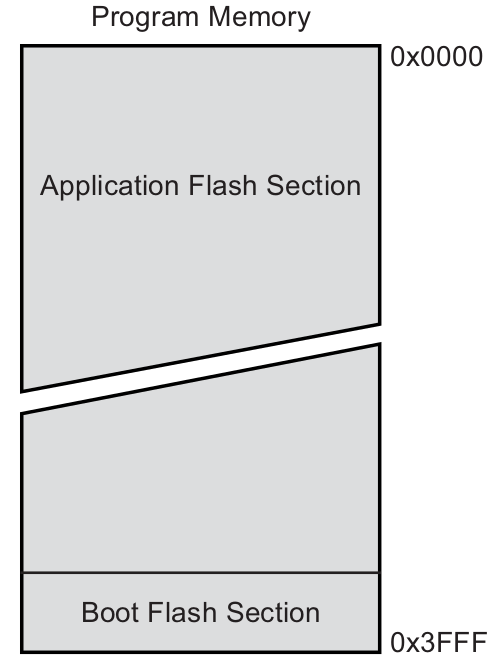
\includegraphics[height=0.27\textheight]{programMemoryFlash.png}
    \end{center}
\end{figure}

\subsection{SRAM Data Memory}
\begin{itemize}
    \item The ATmega328P is a complex microcontroller with more peripheral units than can be supported within the 64 locations reserved in the opcode for the IN and OUT instructions.
    \item For the extended I/O space from 0x60 - 0xFF in SRAM, only the ST/STS/STD and LD/LDS/LDD instructions can be used.
    \begin{figure}[H]
        \begin{center}
            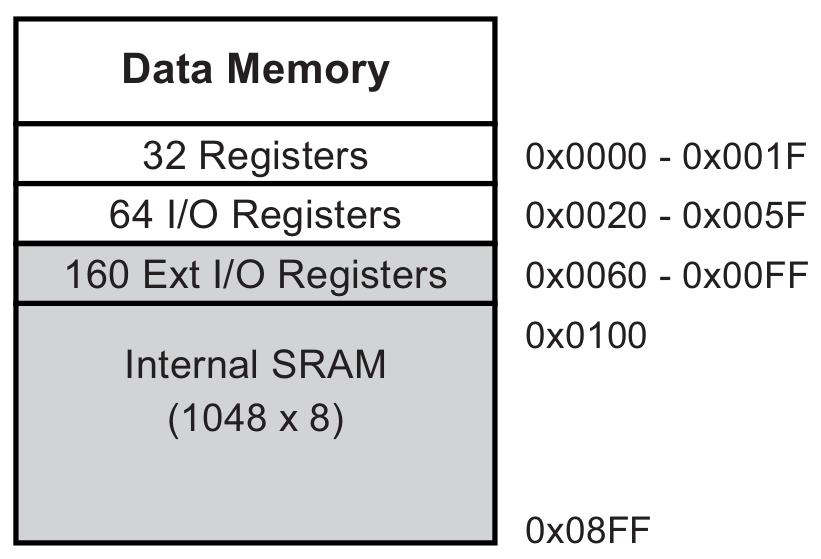
\includegraphics[height=0.25\textheight]{dataMemorySRAM.png}
        \end{center}
    \end{figure}
    \item The lower 2303(0x08FF) data memory locations addresses both the register files, the I/O memory, extended I/O memory and the internal data SRAM.
    \begin{itemize}
        \item The first 32 location addresses the register file.
        \item The next 64 location addresses the standard I/O memory.
        \item The following 160 location address the extended I"O memory.
        \item The last 2048 location address the internal data SRAM.
    \end{itemize}
\end{itemize}

\subsection{EEPROM Data Memory}
\begin{itemize}
    \item 1 K Byte of data EEPROM memory.
    \item Organized as seperate data space.
    \item Endurance of atleast 100,000 write/erase cycle.
    \item EEPROM are accessible in I/O space.
    \item Specific Write procedure is followed. 
\end{itemize}

\subsection{I/O Memory}
\begin{itemize}
    \item I/O and peripherals are placed in the I/O spaces.
    \item All I/O locations are accesed by LD/LDS/LDD and ST/STS/STD instructions.
    \item The I/O registers withing 0x00 - 0x1F are directly bit-accessible using SBI and CBI Instructions.
\end{itemize}


\section{System Clock and Clock Options}
\begin{figure}[H]
    \begin{center}
        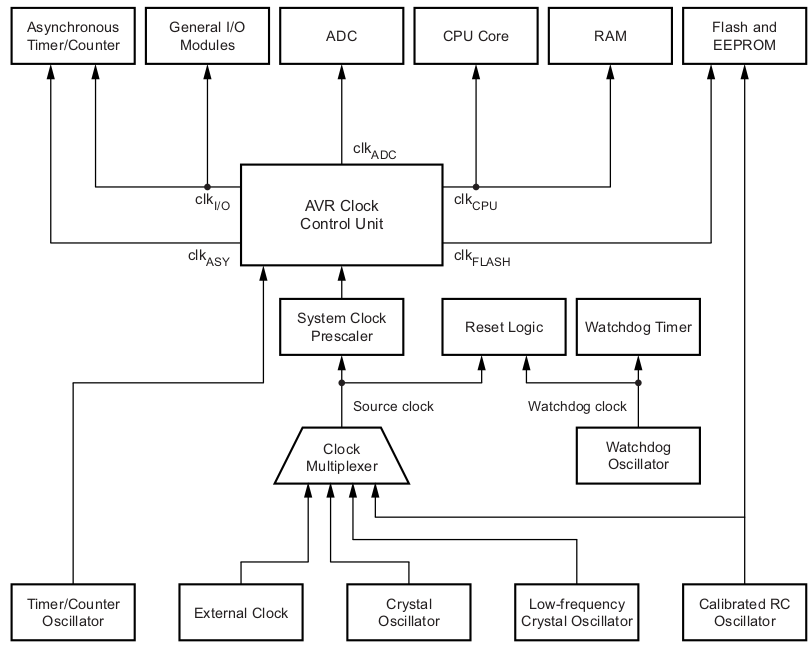
\includegraphics[height=0.5\textheight]{clkDistribution.png}
    \end{center}
\end{figure}

\subsection{Clock Systems}
\subsubsection{CPU Clock}
\begin{itemize}
    \item $clk_{CPU}$ is routed to all parts of AVR core.
    \item General purpose register file, Status register and data memory holding stack pointer.
    \item Halting CPU clock will inhibts the core from perfrorming general operations and caluclations.
\end{itemize}

\subsubsection{I/O Clock}
\begin{itemize}
    \item $clk_{I/O}$ is used in I/O modules like Timers/Counter, SPI, USART, etc.
    \item For external interrupt module also but some external interrupts are detected by asynchonous logic and can be used even when I/O clock is halted.
\end{itemize}

\subsubsection{Flash Clock}
\begin{itemize}
    \item $clk_{FLASH}$ controls operation of flash interface.
\end{itemize}


\subsubsection{Asynchronous Timer Clock}
\begin{itemize}
    \item $clk_{ASY}$ allows asynchonous Timer/Counter to be clocked directly from external clock or an external 32 kHz clock crystall.
    \item This clock allows using Timer/COunter as real-time counter even when device is in sleep mode.
\end{itemize}

\subsubsection{ADC Clock}
\begin{itemize}
    \item $clk_{ADC} had dedicated clock domain$
    \item Gives more accurate ADC conversion result
\end{itemize}

\subsection{Clock Sources}
\quad Selectable clock sources using flash fuse bits.

\begin{table}[H]
    \begin{center}
        \begin{tabular}{c|c}
            \textbf{\bitFormat{CKSEL[3:0]}} & \textbf{Device Clocking Option}\\
            \hline
            1111 - 1000 & Low power crystall oscillator\\
            0111 - 0110 & Full swing crystal oscillator\\
            0101 - 0100 & Low frequency crystal oscillator\\
            0011 & Internal 128kHz RC oscillator\\
            0010 & Calibrated internal RC oscillator\\
            0000 & External clock            
        \end{tabular}
    \end{center}
\end{table}

{\Large \textbf{For fuses, "1" denotes unprogrammed and "0" denotes programmed.}}

\subsubsection*{Default Clock Source}
\begin{itemize}
    \item Devices is shipped with interface RC oscillator at 8.0MHz with fuse \bitFormat{CKDIV8} programmed meaning $---->$ the internal oscillator produces a 8.0 Mhz clock but due to \bitFormat{CKDIV8} being programmed the system clock gets $\frac{8.0 MHz}{8} = 1 MHz$.
    \item The startup time is set to maximum and time-out period enabled.
    \item Default configuration $--->$ \bitFormat{CKSEL} = 0010; \bitFormat{SUT} = 10; \bitFormat{CKDIV8} = 0.
\end{itemize}

\subsubsection*{Clock Start Sequence}
\begin{itemize}
    \item Clock Source needs a sufficient $V_{CC}$ and minimum number of oscillating cycles before stablizing.
    \item To ensure sufficient $V_{CC}$, the device issues an internal reset with time-out delay ($t_{TOUT}$).
    \item The number of cyles in the dealy is set by \bitFormat{SUTx} bits and \bitFormat{CKSELx} fuse bits.
    \item The main purpose of dealy is to keep AVR in reset until it is supplied with minimal $V_{CC}$.
    \item The start-up sequence for the clock includes both the time-out delay and the start-up time when the device starts up from
    reset.
\end{itemize}

\subsubsection*{Clock Output Buffer}
\begin{itemize}
    \item device can output system clock on the \pinFormat{CLKO} pin.
    \item enabled by \pinFormat{CKOUT} fuse.
    \item any clock source can be used to output from this pin.
\end{itemize}

\subsubsection*{TIMER/COUNTER OSCILLATOR}
\begin{itemize}
    \item uses the same crystal oscillator for low-frequency oscillator and Timer/Counter oscillator.
    \item Since, It shares the Timer/Counter oscillator pins  \pinFormat{TOSC1} and \pinFormat{TOSC2} pins with \pinFormat{XTAL1} and \pinFormat{XTAL2}, the system clock must be four times the oscillator and so the Timer/Counter oscillator can only be used when the calibrated internal RC oscillator is selected as system clock source.
\end{itemize}

\subsubsection{Low Power Crystall OSscillator}

\begin{figure}[H]
	\begin{minipage}{.45\textwidth}
		\begin{center}
			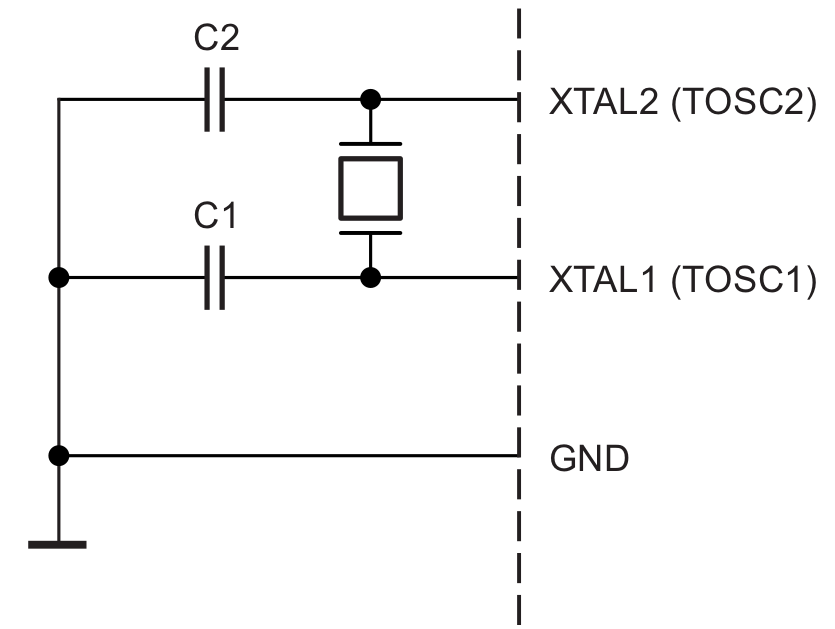
\includegraphics[width=0.45\textwidth]{lowPowerCrystallOscillatorCircuit.png}
			\caption{VGA Connector}
		\end{center}
	\end{minipage}
	\begin{minipage}{.5\textwidth}
		\begin{center}
			\begin{tabular}{c|c}
                \bitFormat{CKSEL[3:1]} & \textbf{Frequency Range (MHz)}\\
                \hline
                100 & 0.4 to 0.9(only Ceramic resonators)\\
                101 & 0.9 to 3.0\\
                110 & 3.0 to 8.0\\
                111 & 8.0 to 16.0\\
            \end{tabular}
		\end{center}
	\end{minipage}
\end{figure}


\begin{itemize}
    \item \pinFormat{XTAL1} and \pinFormat{XTAL2} are inputs and outpus of an inverting amplifier which can be configured as on-chip oscillator.
    \item Either Quartz Crystall or Ceramic resonator can be used.
    \item Crystal Oscillator is a low power oscillator with reduced voltage swing on the XTAL2 output.
    \item Not capable of driving other clock inputs.
    \item C1 and C2 should be of the same values – 12pF to 22pF.
    \item The \bitFormat{CKSEL[0]} fuse together with the \bitFormat{SUT[1:0]} fuses select the start-up times as shown in Table below.
    \begin{figure}[H]
        \begin{center}
            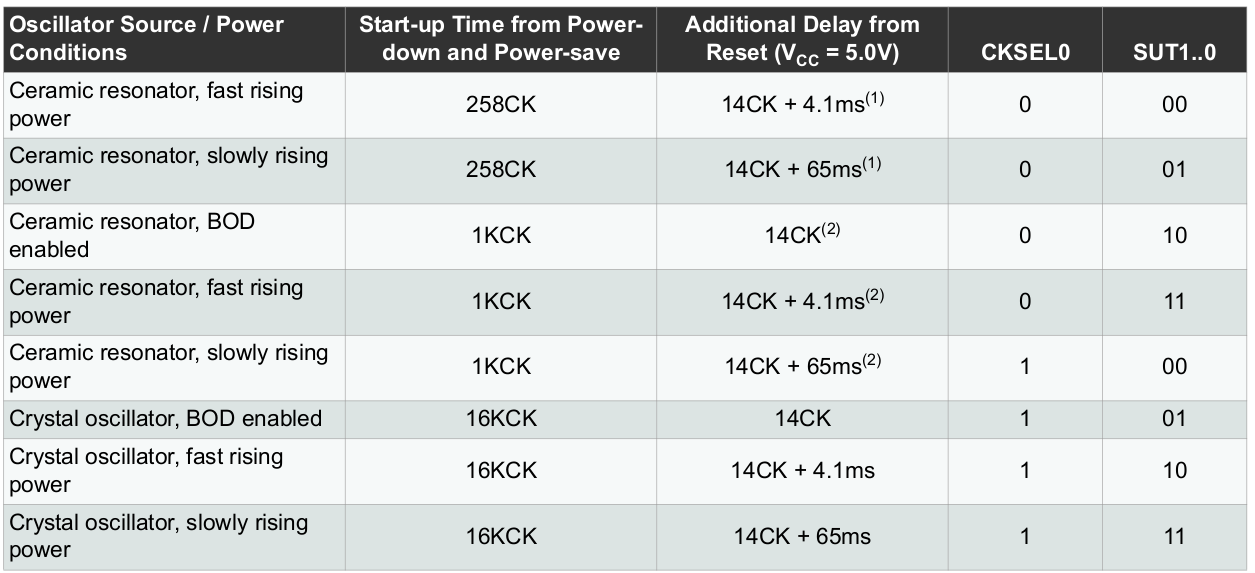
\includegraphics[width=0.95\textwidth]{startUpTimesLowPowerCrystallOscillator.png}
        \end{center}
    \end{figure}
\end{itemize}

\subsubsection{Full Swing Crystal Oscillator}

\begin{figure}[H]
	\begin{minipage}{.45\textwidth}
		\begin{center}
			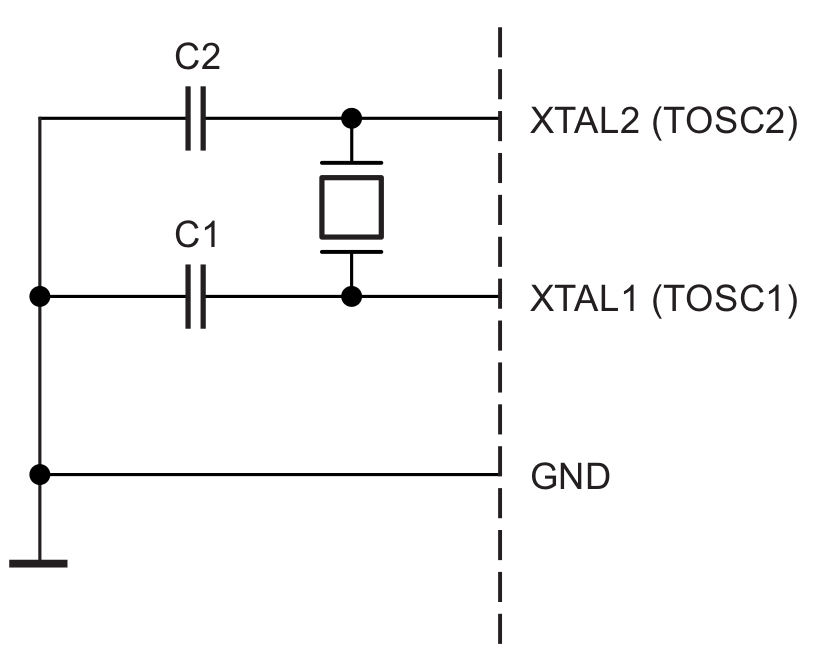
\includegraphics[width=0.45\textwidth]{fullSwingCrysallOscillatorCircuit.png}
			\caption{VGA Connector}
		\end{center}
	\end{minipage}
	\begin{minipage}{.5\textwidth}
		\begin{center}
            \begin{tabular}{c|c}
                \bitFormat{CKSEL[3:1]} & \textbf{Frequency Range (MHz)}\\
                \hline
                011 & 0.4 to 16.0\\
            \end{tabular}
		\end{center}
	\end{minipage}
\end{figure}


\begin{itemize}
    \item \pinFormat{XTAL1} and \pinFormat{XTAL2} are inputs and outpus of an inverting amplifier which can be configured as on-chip oscillator.
    \item Either Quartz Crystall or Ceramic resonator can be used.
    \item Full-Swing with rail-to-rail swing on the XTAL2 outtput.
    \item Can drive other clock input
    \item Power consumption is more than Low power crystal oscillator
    \item Needs $V_{CC}$ = 2.7 to 5.5V
    \item C1 and C2 should be of the same values – 12pF to 22pF.
    \item  The \bitFormat{CKSEL[0]} fuse together with the \bitFormat{SUT[1:0]} fuses select the start-up times as shown in Table below.
    \begin{figure}[H]
        \begin{center}
            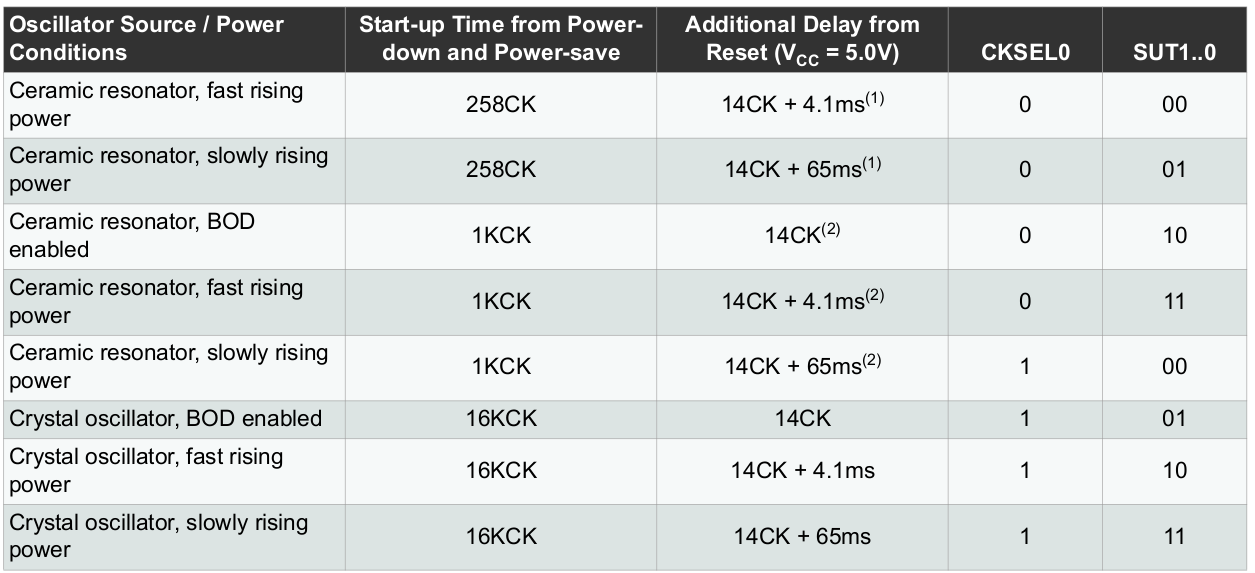
\includegraphics[width=0.95\textwidth]{startUpTimesLowPowerCrystallOscillator.png}
        \end{center}
    \end{figure}
\end{itemize}

\subsubsection{Low Frequency Crystal Oscillator}
\begin{itemize}
    \item To use with 32.765kHz watch crystal
    \item Crystal Cap(CL) – 6.5,9.0 and 12.5pF
    \item \bitFormat{CKSEL[3:0]} == 0101.
    \item The Start-up Times for the Low-frequency Crystal O scillator Clock Selection
    \begin{figure}[H]
        \begin{center}
            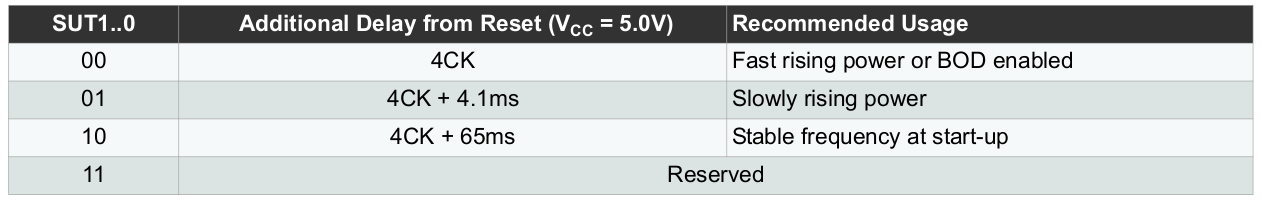
\includegraphics[width=0.95\textwidth]{startUpTimelowFrequencyCrysalOscillator.png}
        \end{center}
    \end{figure}
\end{itemize}

\subsubsection{Calibrated Internal RC Oscillator}
\begin{itemize}
    \item 8.0MHz clock
    \item Voltage and temperature dependent
    \item Calibration is done in \regFormat{OSCCAL}.
    \item Default mode shipeed with CKDIV8 prescalar programmed to prescale causing the system clock to be 1.0MHz.
    \item \bitFormat{CKSEL[3:0]} == 0010.
    \begin{figure}[H]
        \begin{center}
            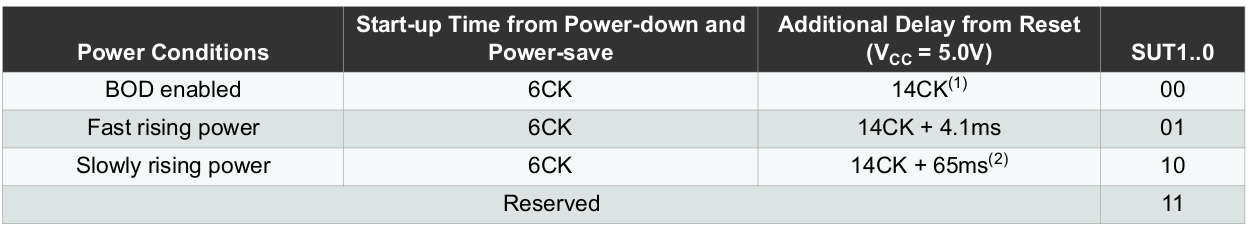
\includegraphics[width=0.95\textwidth]{startUpTimeCalibratedInternalRCOscillator.png}
        \end{center}
    \end{figure}
\end{itemize}

\subsubsection{128kHz Internal Oscillator}
\begin{itemize}
    \item low power oscillator with 128kHz frequency
    \item \bitFormat{CKSEL[3:0]} == 0010.
    \begin{figure}[H]
        \begin{center}
            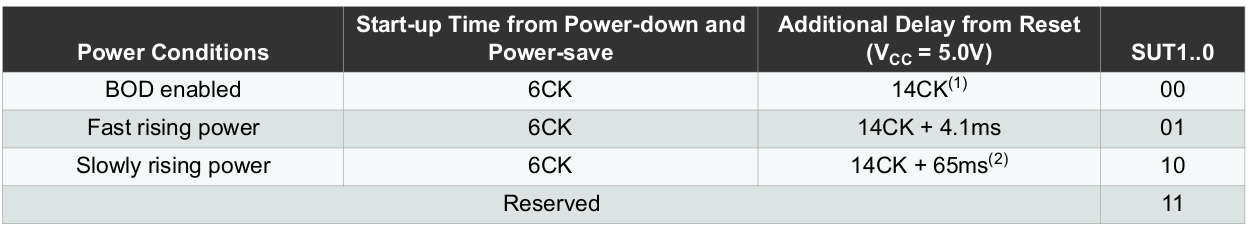
\includegraphics[width=0.95\textwidth]{startUpTimeCalibratedInternalRCOscillator.png}
        \end{center}
    \end{figure}
\end{itemize}

\subsubsection{External Clock}
\begin{figure}[H]
    \begin{center}
        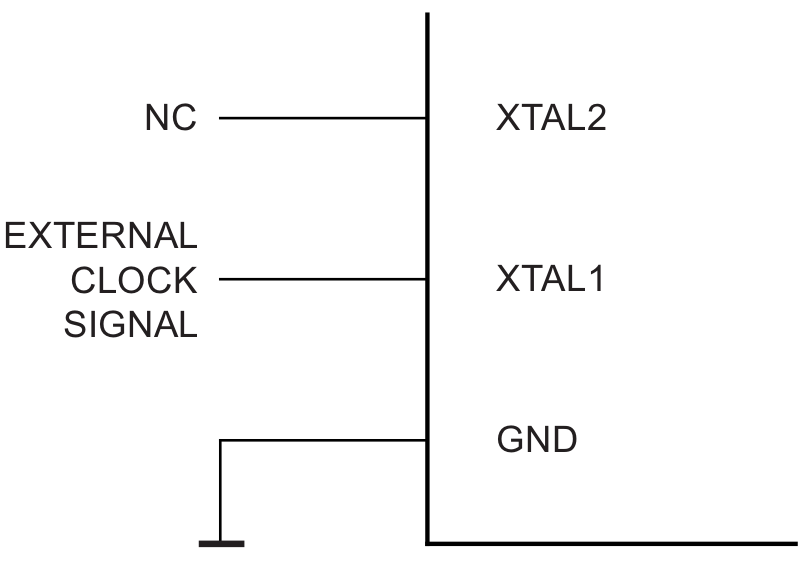
\includegraphics[width=0.25\textwidth]{externalClockciruit.png}
    \end{center}
\end{figure}
\begin{itemize}
    \item XTAL1 must be connected to external source.
    \item 0 - 16 MHz frequency.
    \item \bitFormat{CKSEL} == 0000.
    \item Start-up times are determined by the SUT fuses as
    \begin{figure}[H]
        \begin{center}
            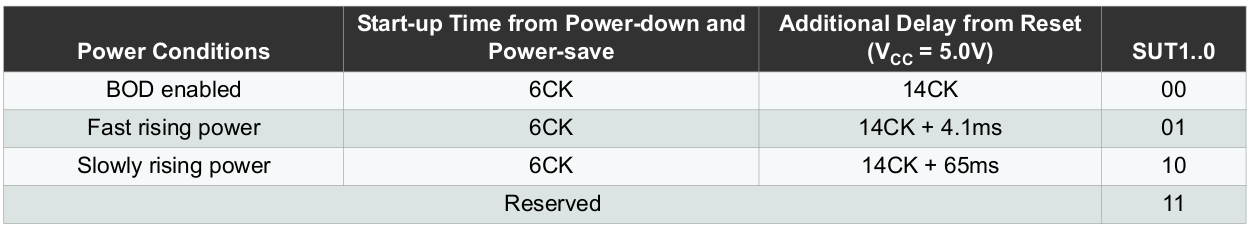
\includegraphics[width=0.95\textwidth]{startUpTimeExternalClock.png}
        \end{center}
    \end{figure}
\end{itemize}

\subsection{System Clock Prescalar}
\begin{itemize}
    \item The system clock can be divided by setting the \regFormat{CLKPR} (Clock Prescale Registers) value.
    \item Used to decrease the system clock frequency and the power consumption when the requirement for processing power is low.
    \item Affects the $clk_{SYS}$, $clk_{IO}$, $clk_{ADC}$, $clk_{CPU}$ and $clk_{FLASH}$.
    \item A special write procedure is followed to change \bitFormat{CLKPS} bits:
    \begin{enumerate}[label=(\roman*)]
        \item Write the clock prescaler change enable (\bitFormat{CLKPCE}) bit to one and all other bits in \regFormat{CLKPR} register to zero.
        \item Within four cycles, write the desired value to \bitFormat{CLKPS} bit while writing a zero to \bitFormat{CLKPCE}.
        \item Interrupt must be disabled.
    \end{enumerate}
\end{itemize}

\subsubsection{Register Description}
\subsubsection*{OSCCAL – Oscillator Calibration Register}
\vspace*{0.5cm}
\begin{bytefield}[bitformatting={\large\bfseries},
    endianness=big,bitwidth=0.125\linewidth]{8}
    \bitheader[lsb=0]{0-7} \\
    \bitbox{1}{\small CAL7}
    \bitbox{1}{\small CAL6}
    \bitbox{1}{\small CAL5}
    \bitbox{1}{\small CAL4}
    \bitbox{1}{\small CAL3}
    \bitbox{1}{\small CAL2}
    \bitbox{1}{\small CAL1}
    \bitbox{1}{\small CAL0}\\
\end{bytefield}
\begin{itemize}
    \item The oscillator calibration register is used to trim the calibrated internal RC oscillator to remove process variations from the oscillator frequency.
    \item A pre-programmed calibration value is automatically written to this register during chip reset.
    \item The application software can write this register to change the oscillator frequency.
    \item If EEPROM is to be used, shouldn't do calibration for more than 8.8 MHz.
    \item \bitFormat{CAL7} bit detected range of operation of oscillator. Setting zeros gives the Lowest requency range, setting this bit to 1 gives the highest frequency range.
    \item The \bitFormat{CAL[6:0]} bits are used to tune the frequency within the selected range. A setting of 0x00 gives the lowest frequency in that range, and a setting of 0x7F gives the highest frequency in the range.
\end{itemize}

\subsubsection*{CLKPR – Clock Prescale Register}
\vspace*{0.5cm}
\begin{bytefield}[bitformatting={\large\bfseries},
    endianness=big,bitwidth=0.125\linewidth]{8}
    \bitheader[lsb=0]{0-7} \\
    \bitbox{1}{\small CLKPCE}
    \bitbox{1}{\small -}
    \bitbox{1}{\small -}
    \bitbox{1}{\small -}
    \bitbox{1}{\small CLKPS3}
    \bitbox{1}{\small CLKPS2}
    \bitbox{1}{\small CLKPS1}
    \bitbox{1}{\small CLKPS0}\\
\end{bytefield}

\begin{itemize}
    \item \bitFormat{CLKPCE} - Cloc k Prescaler Change Enable must be written to logic one to enable change of the \bitFormat{CLKPS} bits.
    \item The \bitFormat{CLKPCE} bit is only updated when the other bits in CLKPR are simultaneously written to zero.
    
    \begin{table}[H]
        \begin{center}
            \begin{tabular}{c|c}
                \bitFormat{CLKPS[3:0]} & \textbf{Clock Division Facter}\\
                \hline
                0000 & 1\\
                0001 & 2\\
                0010 & 4\\
                0011 & 8\\
                0100 & 16\\
                0101 & 32\\
                0110 & 64\\
                0111 & 128\\
                1000 & 256\\                
            \end{tabular}
        \end{center}
    \end{table}

    \item \bitFormat{CLKPS[3:0]} - Clock Prescaler Select Bits define the division factor between the selected clock source and the internal system clock.
    \item The \bitFormat{CKDIV8} fuse determines the initial value of the \bitFormat{CLKPS} bits. 
    \begin{itemize}
        \item If \bitFormat{CKDIV8} is unprogrammed, the \bitFormat{CLKPS} bits will be reset to 0000.
        \item If \bitFormat{CKDIV8} is programmed, \bitFormat{CLKPS} bits are reset to “0011”, giving a division factor of 8 at start up.
    \end{itemize} 
    \item Note that any value can be written to the \bitFormat{CCLKPS} bits regardless of the \bitFormat{CCKDIV8} fuse setting.
\end{itemize}

\section{Power Management and Sleep modes}
\begin{itemize}
    \item Sleep modes enable the application to shut down unused modules in the MCU, thereby saving power.
    \item When enabled, the brown-out detector (BOD) actively monitors the power supply voltage during the sleep periods.
    \item To further save power, it is possible to disable the BOD in some sleep modes.
\end{itemize}

\subsection{Sleep Modes}
\begin{itemize}
    \item To enter any of the six sleep modes, the \bitFormat{SE} bit in \regFormat{SMCR} register must be written to logic one.
    \item The \bitFormat{SM[2:0]} bits in the \regFormat{SMCR} register select which sleep mode.
    \item \emph{SLEEP} instruction must be executed.
    \item If an enabled interrupt occurs while the MCU is in a sleep mode, the MCU wakes up.
    \item The MCU is then halted for four cycles in addition to the start-up time, executes the interrupt routine, and resumes execution from the instruction following SLEEP.
    \item The contents of the register file and SRAM are unaltered when the device wakes up from sleep. 
    \item If a reset occurs during sleep mode, the MCU wakes up and executes from the reset vector.
    \item The Active Clock Domains and Wake-up Sources in the Different Sleep Modes,
\end{itemize}
\begin{figure}[H]
    \begin{center}
        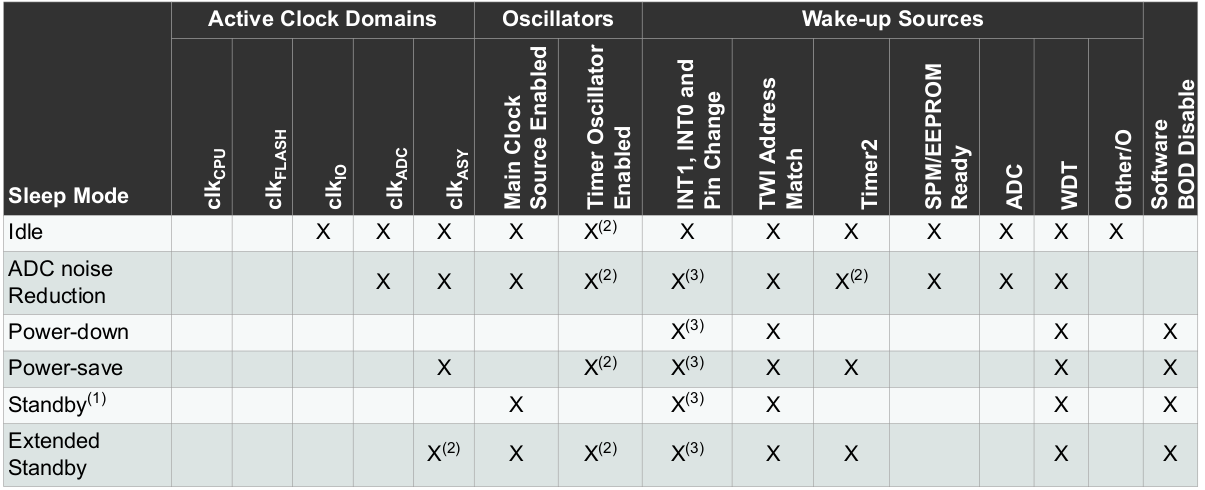
\includegraphics[width=1\textwidth]{sleepModeDomain.png}
    \end{center}
\end{figure}

\subsubsection{Idle Mode}
\begin{itemize}
    \item Stops the CPU but allows the SPI, USART, analog comparator, ADC, 2-wire serial interface, Timer/Counters, watchdog, and the interrupt
    system.
    \item Halts $clk_{CPU}$ and  $clk_{FLASH}$ and allows other clocks.
    \item Idle mode enables the MCU to wake up from external triggered interrupts as well as internal ones like the timer overflow and USART transmit complete interrupts.
\end{itemize}

\subsubsection{ADC Noise Reduction Mode}
\begin{itemize}
    \item Stops the CPU but allows ADC, the external interrupts, the 2-wire serial interface address watch, Timer/Counter2 and the watchdog.
    \item Halts $clk_{I/O}$, $clk_{CPU}$ and  $clk_{FLASH}$ and allows other clocks.
    \item Improves the noise environment for ADC, enabling higher resolution measurement.
    \item ADC Noise Reduction Mode enables the MCU to wake up from external reset, a watchdog system reset, a watchdog interrupt, a brown-out reset, a 2-wire serial interface address match, a Timer/Counter2 interrupt, an SPM/EEPROM ready interrupt, an external level interrupt on INT0 or INT1 or a pin change interrupt.
\end{itemize}

\subsubsection{Power-down Mode}
\begin{itemize}
    \item Stops the external oscillator but allows the external interrupts, the 2-wire serial interface address watch, and the watchdog.
    \item Halts all clocks and asynchronous modules only.
    \item Power-down mode enables the MCU to wake up from an external reset, a watchdog system reset, a watchdog interrupt, a brown-out reset, a 2-wire serial interface address match, an external level interrupt on INT0 or INT1, or a pin change interrupt.
\end{itemize}


\subsubsection{Power-save Mode}
\begin{itemize}
    \item Only diffence from Power-down mode is Timer/Counter2 is enabled and it will run.
    \item Timer overflow or output compare event from Timer/Counter2 can wake up.
\end{itemize}

\subsubsection{Standby Mode}
\begin{itemize}
    \item Selects the external crystal clock option.
    \item Identical to power-down except oscillator is running.
\end{itemize}

\subsubsection{External Standby Mode}
\begin{itemize}
    \item Selects the external crystal clock option.
    \item Identical to power-Save except oscillator is running.
\end{itemize}

\subsubsection{Register Description}
\subsubsection*{SMCR – Sleep Mode Control Register}
\vspace*{0.5cm}
\begin{bytefield}[bitformatting={\large\bfseries},
    endianness=big,bitwidth=0.125\linewidth]{8}
    \bitheader[lsb=0]{0-7} \\
    \bitbox{1}{\small -}
    \bitbox{1}{\small -}
    \bitbox{1}{\small -}
    \bitbox{1}{\small -}
    \bitbox{1}{\small SM2}
    \bitbox{1}{\small SM1}
    \bitbox{1}{\small SM0}
    \bitbox{1}{\small SE}\\
\end{bytefield}

\begin{table}[H]
    \begin{center}
        \begin{tabular}{c|c}
            \bitFormat{SM[2:0]} & \textbf{Sleep Mode}\\
            \hline
            000 & Idle\\
            001 & ADC Noise Reduction\\
            010 & Power-down\\
            011 & Power-save\\
            110 & Standby\\
            111 & External Standby\\
        \end{tabular}
    \end{center}
\end{table}
\begin{itemize}
    \item \bitFormat{SE} bit must be written to logic one  just before the SLEEP instruction is executed, to make the MCU enter the sleep mode.
\end{itemize}

\subsection{Power Reduction Register}
\begin{itemize}
    \item To stop the clock to individual peripherals to reduce power consumption.
    \item The current state of the peripheral is frozen and the I/O registers can not be read or written.
    \item Peripheral should in most cases be disabled before stopping the clock.
    \item Wake up peripherals can be done by writing zero to bits in \regFormat{PRR}.
\end{itemize}

\subsubsection{Register Description}
\subsubsection*{PRR – Power Reduction Register}
\vspace*{0.5cm}
\begin{bytefield}[bitformatting={\large\bfseries},
    endianness=big,bitwidth=0.125\linewidth]{8}
    \bitheader[lsb=0]{0-7} \\
    \bitbox{1}{\small PRTWI}
    \bitbox{1}{\small PRTIM2}
    \bitbox{1}{\small PRTIM0}
    \bitbox{1}{\small -}
    \bitbox{1}{\small PRTIM1}
    \bitbox{1}{\small PRSPI}
    \bitbox{1}{\small PRUSART0}
    \bitbox{1}{\small PRADC}\\
\end{bytefield}


\begin{table}[H]
    \begin{center}
        \begin{tabular}{c|c}
            \textbf{Bits} & \textbf{Name}\\
            \hline
            \bitFormat{PRTWI} & Power Reduction TWI\\
            \bitFormat{PRTIM2} & Power Reduction Timer/Counter2\\
            \bitFormat{PRTIM1} & Power Reduction Timer/Counter1\\
            \bitFormat{PRTIM0} & Power Reduction Timer/Counter0\\
            \bitFormat{PRSPI} & Power Reduction Serial Peripheral Interface\\
            \bitFormat{PRUSART0} & Power Reduction USART0\\
            \bitFormat{PRADC} & Power Reduction ADC\\
        \end{tabular}
    \end{center}
\end{table}

\subsection{Minimizing Power Consumption}
\begin{itemize}
    \item In general, sleep modes should be used as much as possible.
    \item ADC should be disabled before entering any sleep mode.
    \item Analog comparator should be disabled in  all sleep modes.
    \item If the brown-out detector is not needed by the application, this module should be turned off by \bitFormat{BODLEVEL} fuses.
    \item If Internal Voltage Reference is not needded and ADC or analog comparator or BOD is not needed, the Internal Voltage Reference can be disabled.
    \item If the watchdog timer is not needed in the application, the module should be turned off.
    \item If On-chip Debug System is not needed, can be disabled by \bitFormat{DWEN} fuse.
    \item For Port pins,
    \begin{itemize}
        \item No pins drive resistive loads.
        \item Input buffers are disabled when I/O clock and ADC clocks are stopped.
        \item If the input buffer is enabled and the input signal is left floating or have an analog signal level close to V CC /2, the input buffer will use excessive power.
        \item Digital input buffers can be disabled by writing to the digital input disable registers (\regFormat{DIDR1} and \regFormat{DIDR0}).
    \end{itemize}
\end{itemize}

\section{RESETTING AVR}
\quad All I/O registers are set to their intial values and program starts execution form reset vector.

\begin{figure}[H]
    \begin{center}
        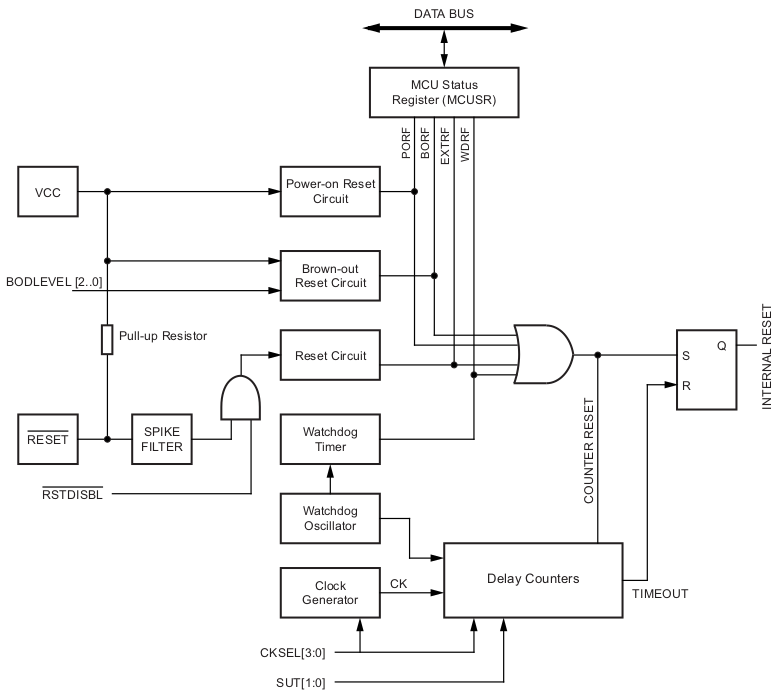
\includegraphics[height=0.55\textheight]{resetLogic.png}
    \end{center}
\end{figure}

\subsection{Reset Sources}
\begin{enumerate}[label=(\Roman*)]
    \item Power-on Reset - MCU resets when supply voltage is below the power-on reset threshold($V_{POT}$).
    \item External Reset - MCU resets when low level is present on \pinFormat{$\overline{RESET}$} is helow for minimum pulse length.
    \item Watchdog System reset - MCU resets when watchdog timer period expires and watchdog system reset mode is enabled.
    \item Brown-out reset - MCU resets when supply voltage $V_{CC}$ is below brown-out threshold ($V_{BOT}$) and brown-out detected is enabled.
\end{enumerate}

\subsubsection{Power-on Reset}
\begin{figure}[H]
    \begin{minipage}{0.45\textwidth}
        \begin{center}
            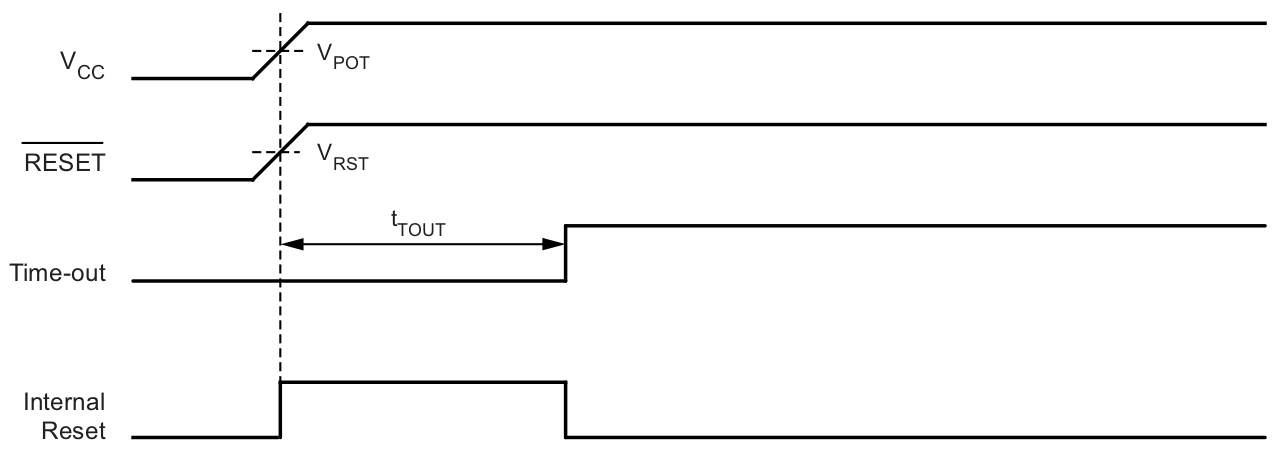
\includegraphics[width=1\textwidth]{POR1.png}
            \caption*{MCU Start-up, $\overline{RESET}$ Tied to $V_{CC}$}
        \end{center}
    \end{minipage}
    \begin{minipage}{0.5\textwidth}
        \begin{center}
            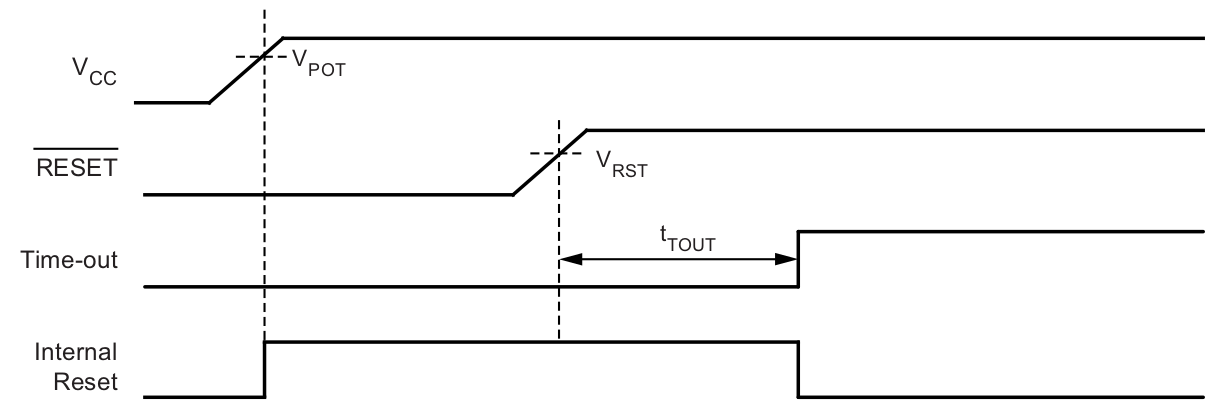
\includegraphics[width=1\textwidth]{POR2.png}
            \caption*{MCU Start-up, $\overline{RESET}$ Extended Externally}
        \end{center}
    \end{minipage}
\end{figure}
\begin{itemize}
    \item A power-on reset (POR) pulse is generated by an on-chip detection circuit.
    \item The POR is activated whenever $V_{CC}$ is below the detection level.
    \item The POR circuit can be used to trigger the start-up reset, as well as to detect a failure in supply voltage.
    \item Reaching the power-on reset threshold voltage invokes the delay counter, which determines how long the device is kept in RESET after $V_{CC}$ rise.
\end{itemize}


\subsubsection{External Reset}
\begin{figure}[H]
    \begin{center}
        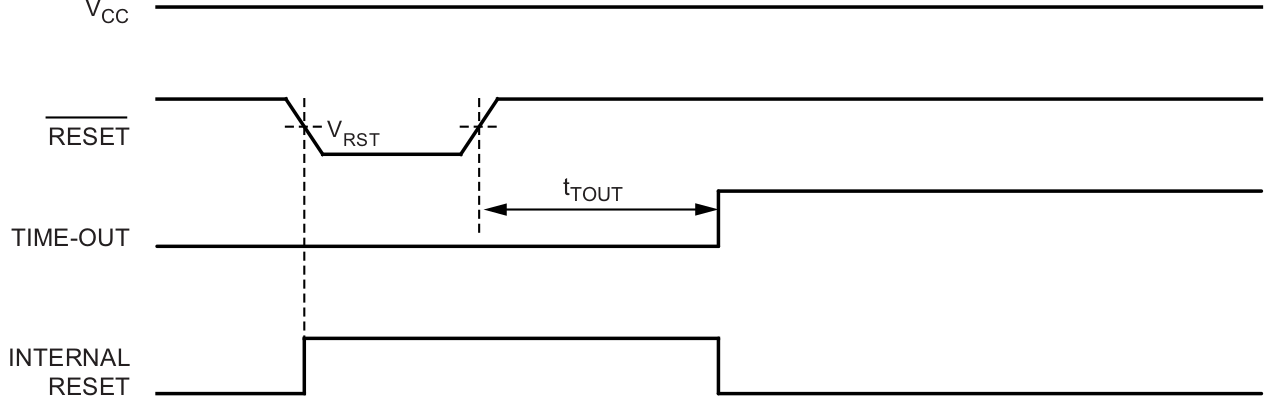
\includegraphics[width=0.5\textwidth]{externalReset.png}
    \end{center}
\end{figure}
\begin{itemize}
    \item An external reset is generated by a low level on the \pinFormat{$\overline{RESET}$}  pin.
    \item Shorter pulses are not guaranteed to generate a reset.
    \item When the applied signal reaches the reset threshold voltage – $V_{RST}$ – on its positive edge, the delay counter starts the MCU after the time-out period – $t_{OUT}$ – has expired.
    \item The external reset can be disabled by the \bitFormat{RSTDISBL} fuse.
\end{itemize}

\subsubsection{Brown-out Detection}
\begin{figure}[H]
    \begin{center}
        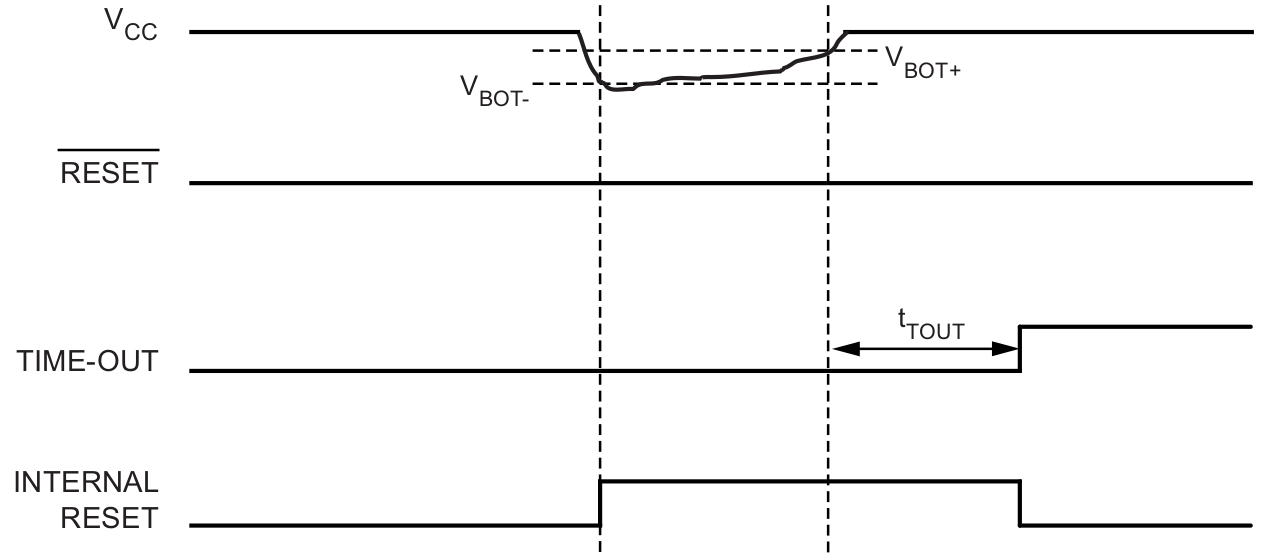
\includegraphics[width=0.5\textwidth]{brownOutReset.png}
    \end{center}
\end{figure}
\begin{itemize}
    \item On-chip brown-out detection (BOD) circuit for monitoring the $V_{CC}$ level during operation by comparing it to a fixed trigger level.
    \item The trigger level for the BOD can be selected by the \bitFormat{BODLEVEL} fuses.
\end{itemize}

\subsubsection{Watchdog System Reset}
\begin{figure}[H]
    \begin{center}
        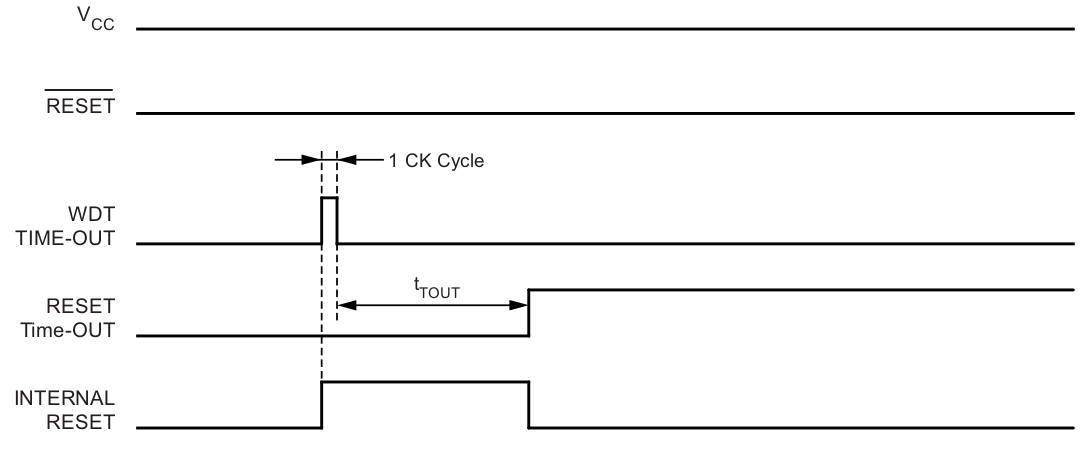
\includegraphics[width=0.5\textwidth]{watchDogReset.png}
    \end{center}
\end{figure}
\begin{itemize}
    \item When the watchdog times out, it will generate a short reset pulse of one CK cycle duration.
    \item On the falling edge of this pulse,
    the delay timer starts counting the time-out period $t_{OUT}$.
\end{itemize}


\end{document}